\newpage
\section{Resultate}

\subsection{Testvoraussetzungen}
Das Netzwerk wurde auf 1'200'000 Bildern des ImageNet-1000-class-Datasets vortrainiert.
Danach wurde es auf rund 13'900 Bildern aus Tabeas Box trainiert. 
Der Test wiederum wurde auf rund 1'500 Bilder ebenfalls aus Tabeas Box getestet. 
Diese Testbilder waren dem Algorithmus während des Lernprozesses nicht zugänglich und haben entsprechend keinen Einfluss auf den Lernprozess genommen. 
Ausserdem wurden diese Bilder so gewählt, dass Sie nicht gleichzeitig aufgenommen wurden. 
Dies verhindert, dass fast identische Bilder im Training und im Test vorkommen. 

\subsection{Analyse}
Um die genauigkeit der Predictions unseres Neuronalen Netzwerkes möglichst genau beschreiben zu können wurden die zwei Werte Distanz und IOU gewählt. 
Obwohl die beiden Werte korrelieren sagt jeder für sich nicht die volle Wahrheit über die Genauigkeit der Vorhersagen aus. 
Die Distanz ist für die geplante Anwendung der wesentlichere Wert, weil diese Informationen über den Standort des Fingers im Bild preisgibt.
Die IOU ist mit der Distanz klar korelliert, denn ist die Distanz zu gross, ist die IOU schnell gleich Null. 
Sobald die Boundingbox der Prediction und die Boundingbox des Labels sich beginnen zu überlappen sagt die IOU etwas über die korrekte Vorhersage von Breite und Höhe der Boundingbox aus. Auch darüber ob die Box am richtigen Ort liegt, können aufgrund der IOU vage Annahmen getroffen werden. Aber wie gesagt, die Distanz ist dafür der sicherere Wert. 

\subsubsection{Distanz}

%Einschätzung der Distanz:
\begin{figure}	
	\centering
	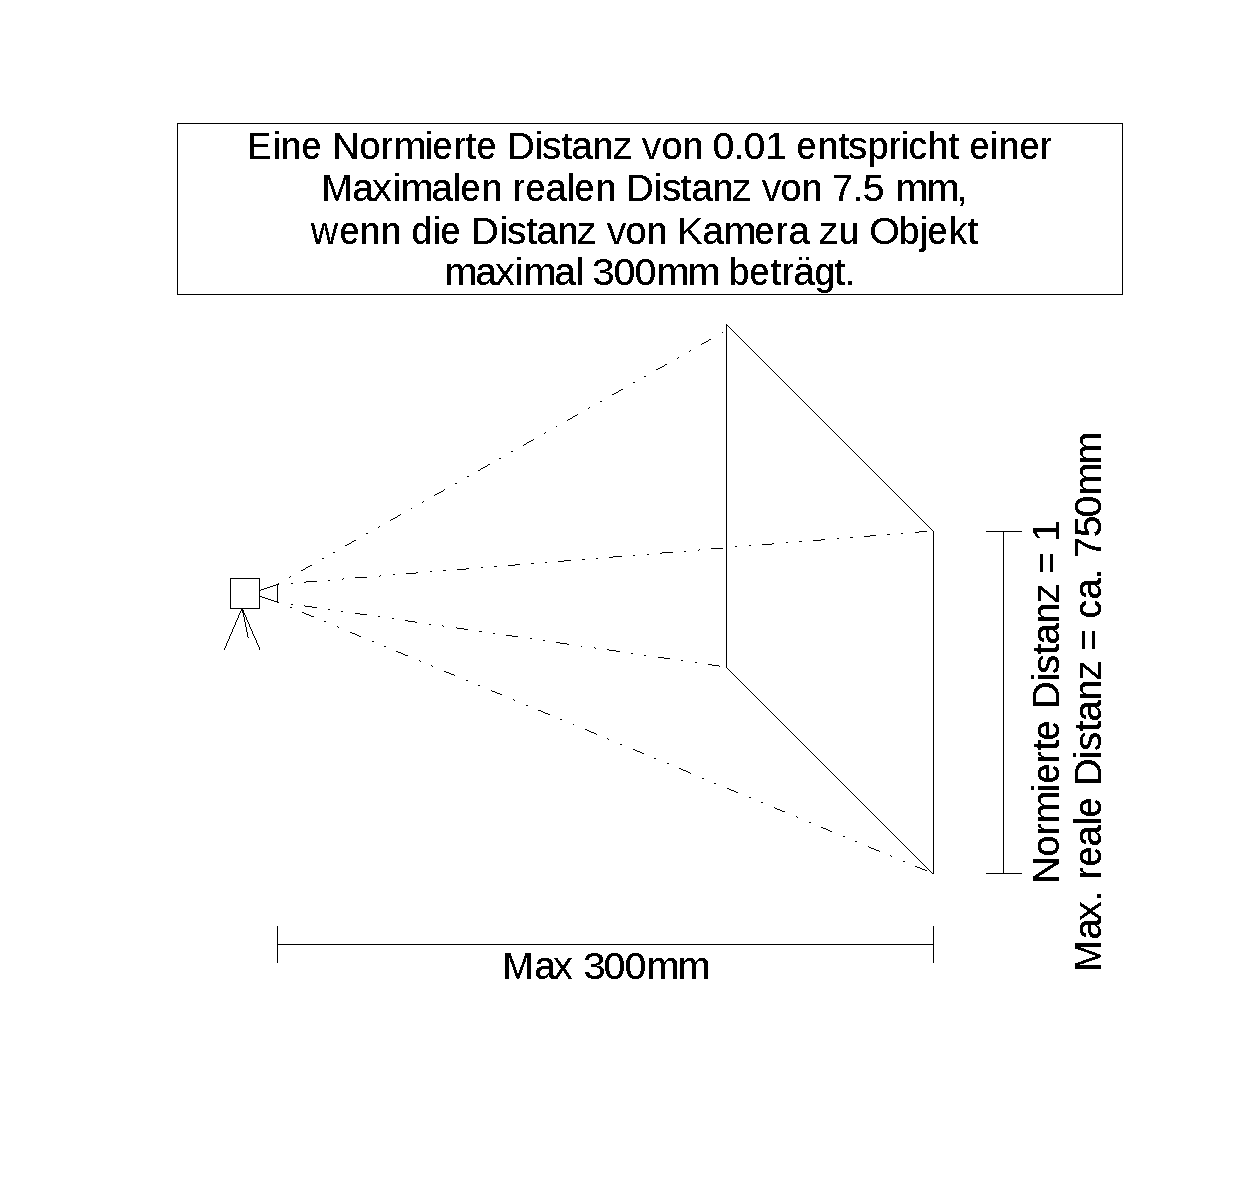
\includegraphics[width=.7\textwidth]{Kapitel/Resultate/Bilder/DistanzenBerechnung.pdf}
	\caption{Bedeutung der normierten Distanzwerte in der realen Welt}
	\label{img:explain_normed_distance}
\end{figure}

%Beispielbilder Distanz
\begin{figure}
	\centering
	\begin{minipage}[b]{0.48\textwidth}	
		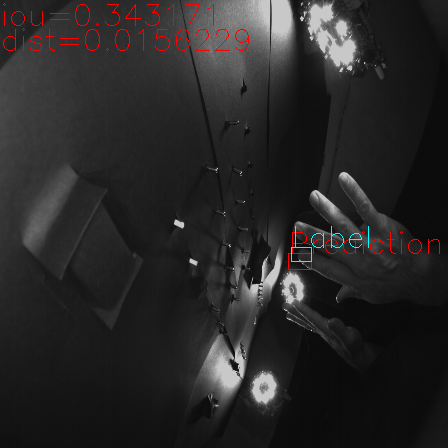
\includegraphics[width=\textwidth]{Kapitel/Resultate/Bilder/2distKnappGut.png}
	\end{minipage}
	\hfill
	\begin{minipage}[b]{0.48\textwidth}		
		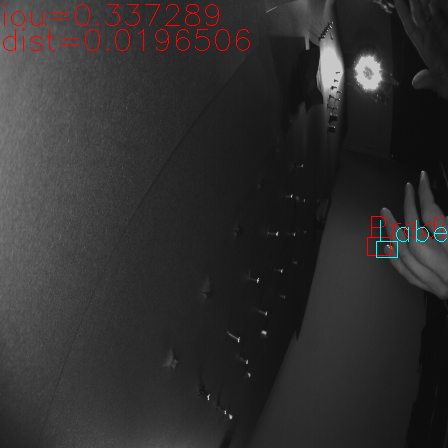
\includegraphics[width=\textwidth]{Kapitel/Resultate/Bilder/5distKnappGut.png}
	\end{minipage}
	\caption{Prediction knapp besser als Distanz=0.02}
	\label{img:distanz_knapp_gut}
	%Eine Leerzeile einfügen	
	\begin{verbatim}
	\end{verbatim}
	\centering
	\begin{minipage}[b]{0.48\textwidth}	
		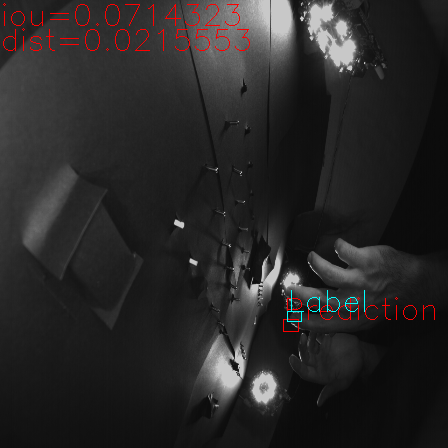
\includegraphics[width=\textwidth]{Kapitel/Resultate/Bilder/3distKnappSchlecht.png}
	\end{minipage}
	\hfill
	\begin{minipage}[b]{0.48\textwidth}		
		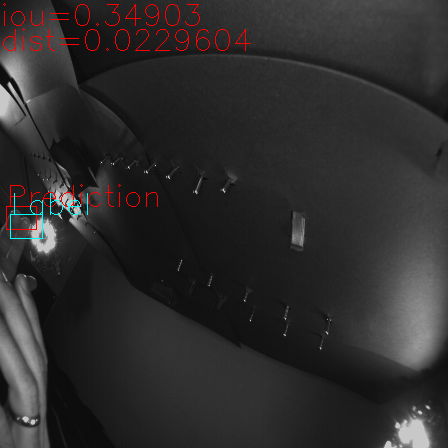
\includegraphics[width=\textwidth]{Kapitel/Resultate/Bilder/4distKnappSchlecht.png}
	\end{minipage}
	\caption{Prediction knapp schlechter als Distanz=0.02}	
	\label{img:distanz_knapp_schlecht}
\end{figure}

%Komplette Wahrscheinlichkeits-Dichte-Funktion der Distanz
\begin{figure}	
	\centering
	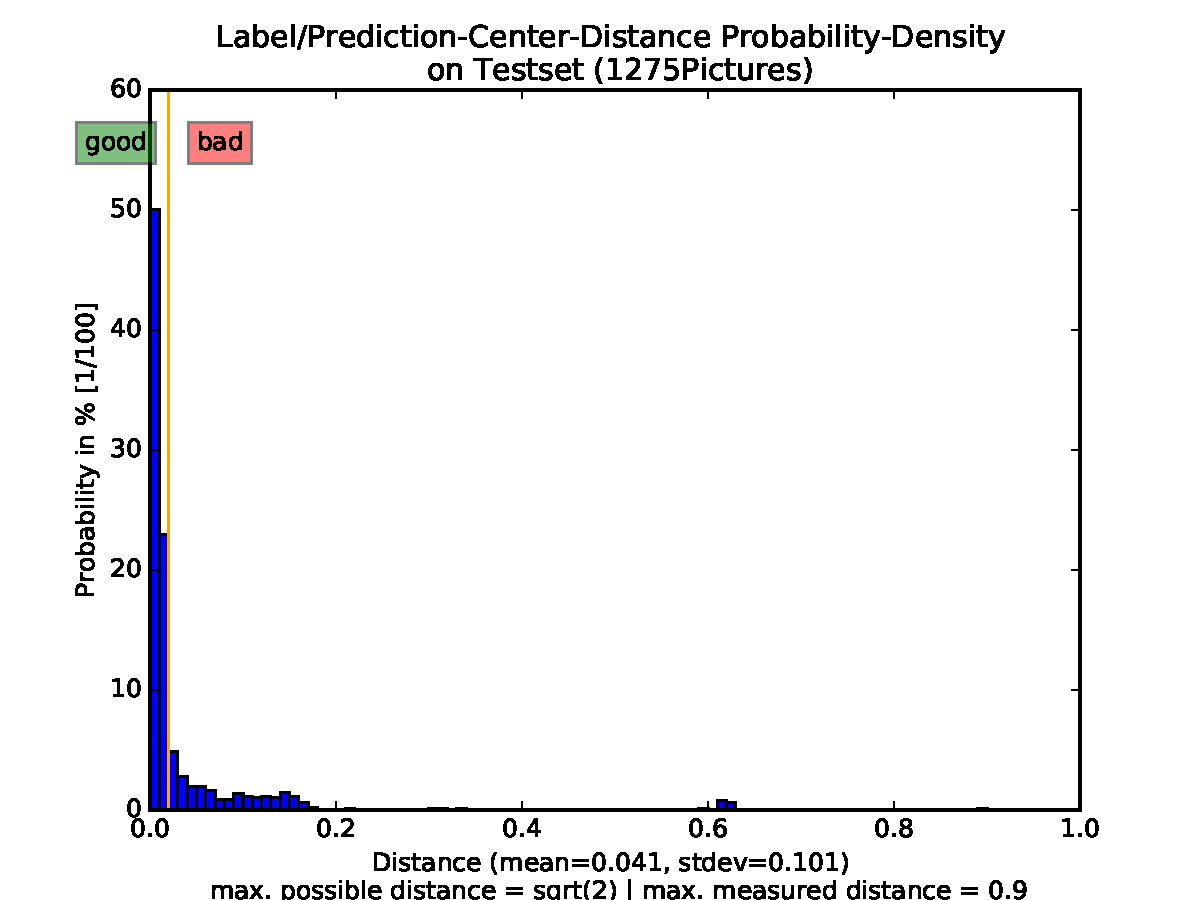
\includegraphics[width=.7\textwidth]{Kapitel/Resultate/Bilder/distProbDensity.pdf}
	\caption{Komplette Wahrscheinlichkeits-Dichte-Funktion der Distanz (Grenze: Dist=0.02)}
	\label{img:dist_dichte}
\end{figure}
%Wahrscheinlichkeits-Dichtefunktion der Distanz. Ausreisser nicht miteingerechnet
\begin{figure}	
	\centering
	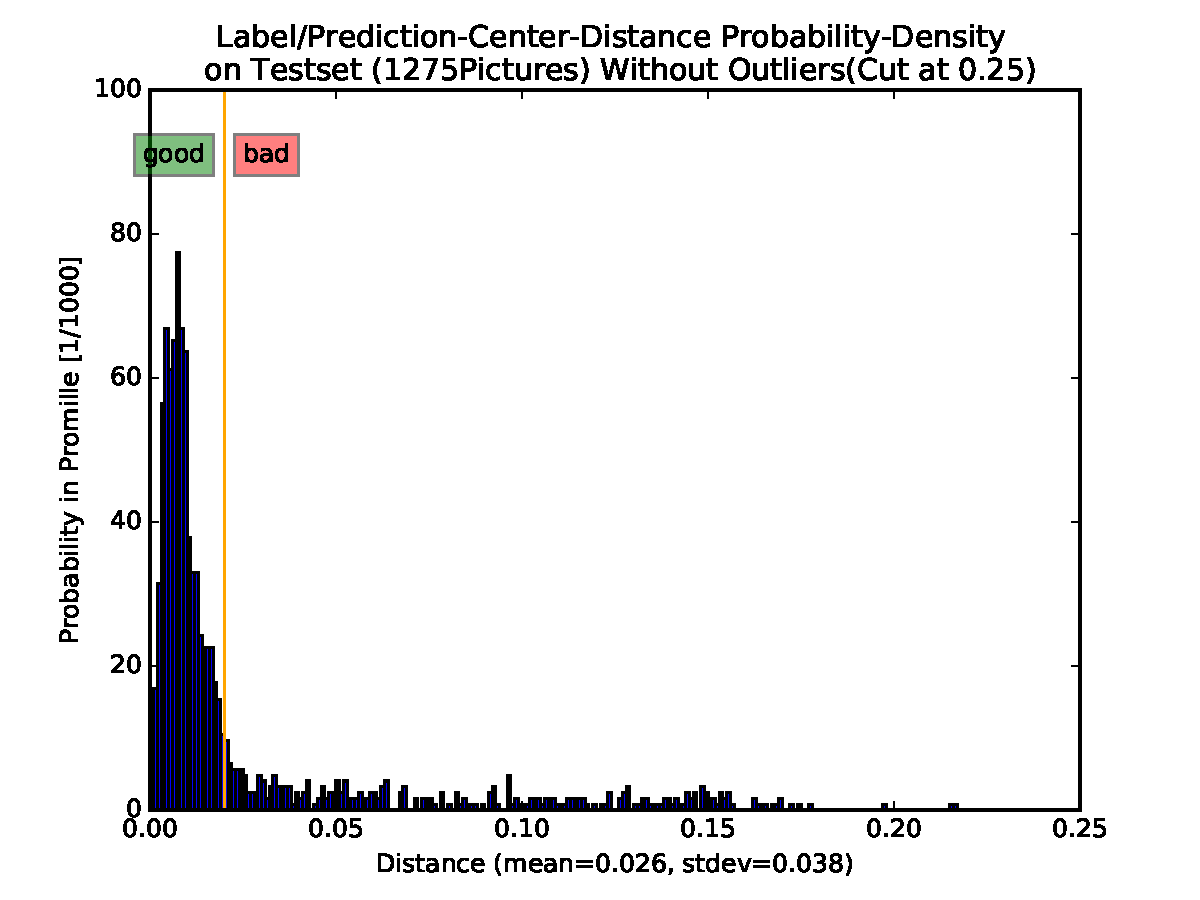
\includegraphics[width=.7\textwidth]{Kapitel/Resultate/Bilder/distProbDensity_improved.pdf}
	\caption{Wahrscheinlichkeits-Dichtefunktion der Distanz. Ausreisser nicht miteingerechnet (Grenze: Dist=0.02)}
	\label{img:dist_dichte_improved}
\end{figure}

Die Distanz beschreibt die normierte Differenz zwischen dem Zentrumspunkt des Labels und dem Zentrumspunkt der Vorhersage. 
Sämtliche Distanzen wurden so normiert, dass die Höhe des Bildes und auch die Breite gleich eins sind. 
Die maximale Distanz zwischen zwei Punkten ist also die Diagonale über ein Bild, welche entsprechend sqrt(2) ist.
Was diese Normierten Distanzen in der realen Welt bedeuten ist auf Abbildung \ref{img:explain_normed_distance} erklärt. 
Zum Vergleich, ein Menschlicher Zeigefinger ist zwischen 10 und 20 mm breit.
Eine normierte Distanz von 0.02 entspricht auf unserem Versuchsaufbau somit ziemlich genau der Breite eines menschlichen Fingers. 

Um die Resultate in gut und schlecht einteilen zu können wurde ein Threshold von 0.02 definiert.
Die Definition dieses Thresholds wurde gemacht, indem Bilder zusammen mit der entsprechenden Distanz analysiert wurden.
Der Wert 0.02 entspricht somit derjenigen Distanz, welche gerade noch knapp annehmbar ist, um einen Finger als detektiert gelten zu lassen.
Um ein Gefühl für diese Distanzen zu kriegen lohnt es sich die Abbildungen \ref{img:distanz_knapp_gut} \& \ref{img:distanz_knapp_schlecht} anzusehen, welche Bilder zeigen, die eine Distanz nahe dieses Thresholds aufweisen. 

Um die Verteilung der Distanzen gut verstehen zu können, ist in Abbildung \ref{img:dist_dichte} eine Wahrscheinlichkeitsdichte der Distanzen im Testset zu sehen. Diese Dichtefunktion wurde erst nach der Bestimmung des Thresholds erzeugt und zeigt, dass rund 73\% der Distanzen kürzer sind als 0.02 und somit die entsprechenden Finger "erfolgreich" erkannt wurden.

Erstaunlich ist auch, dass die Distanzen, welche grösser als 0.25 sind in der Wahrscheinlichkeitsdichte in kleinen Bündeln vorkommen. 
Dies lässt darauf schliessen, dass die trainingsdaten nicht komplett Bias-Frei sind.
Nach kurzer Kontrolle konnte tatsächlich festgestellt werden, dass z.B. bei einer Distanz von 0.6 immer ein bestimmter Punkt des Hintergrundes vorhergesagt wurde, welcher tatsächlich ganz selten in den Labels als Finger markiert wurde. 

Um die Statistik nicht von Ausreissern, welche aufgrund von falschen Labels entstanden sind verfälschen zu lassen, wurde wie in Abbildung \ref{img:dist_dichte_improved} noch eine zweite Wahrscheinlichkeitsdichte-Funktion erstellt. Spannend: Der Mittelwert ist sofort um einen Drittel kleiner als zuvor. 

\subsubsection{Intersection Over Union IOU}
%Beispielbilder IOU
\begin{figure}
	\centering
	\begin{minipage}[b]{0.48\textwidth}	
		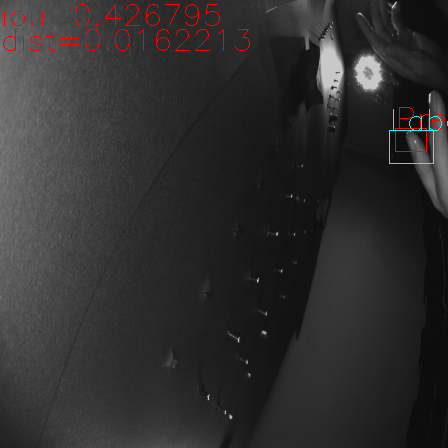
\includegraphics[width=\textwidth]{Kapitel/Resultate/Bilder/7iouKnappGut.png}
	\end{minipage}
	\hfill
	\begin{minipage}[b]{0.48\textwidth}		
		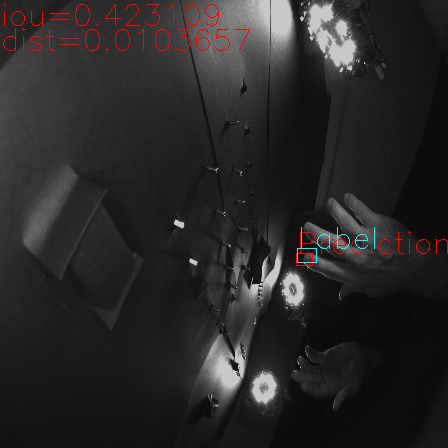
\includegraphics[width=\textwidth]{Kapitel/Resultate/Bilder/8iouKnappGut.png}
	\end{minipage}
	\caption{Prediction knapp besser als IOU=0.4}
	\label{img:iou_knapp_gut}
	%Eine Leerzeile einfügen	
	\begin{verbatim}
	\end{verbatim}
	\centering
	\begin{minipage}[b]{0.48\textwidth}	
		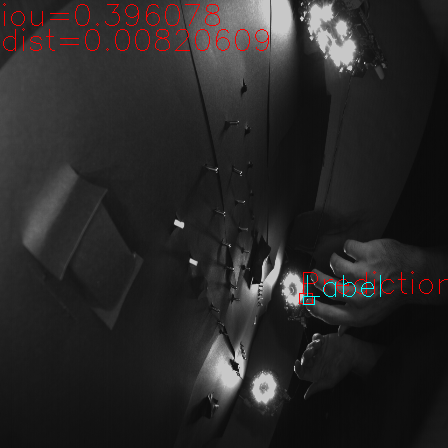
\includegraphics[width=\textwidth]{Kapitel/Resultate/Bilder/6iouKnappSchlecht.png}
	\end{minipage}
	\hfill
	\begin{minipage}[b]{0.48\textwidth}		
		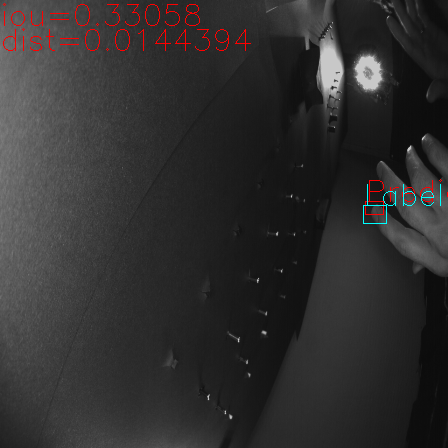
\includegraphics[width=\textwidth]{Kapitel/Resultate/Bilder/9iouKnappSchlecht.png}
	\end{minipage}
	\caption{Prediction knapp schlechter als IOU=0.4}
	\label{img:iou_knapp_schlecht}
\end{figure}
%Wahrscheinlichkeits-Dichte-Funktion der IOU
\begin{figure}
	\centering
	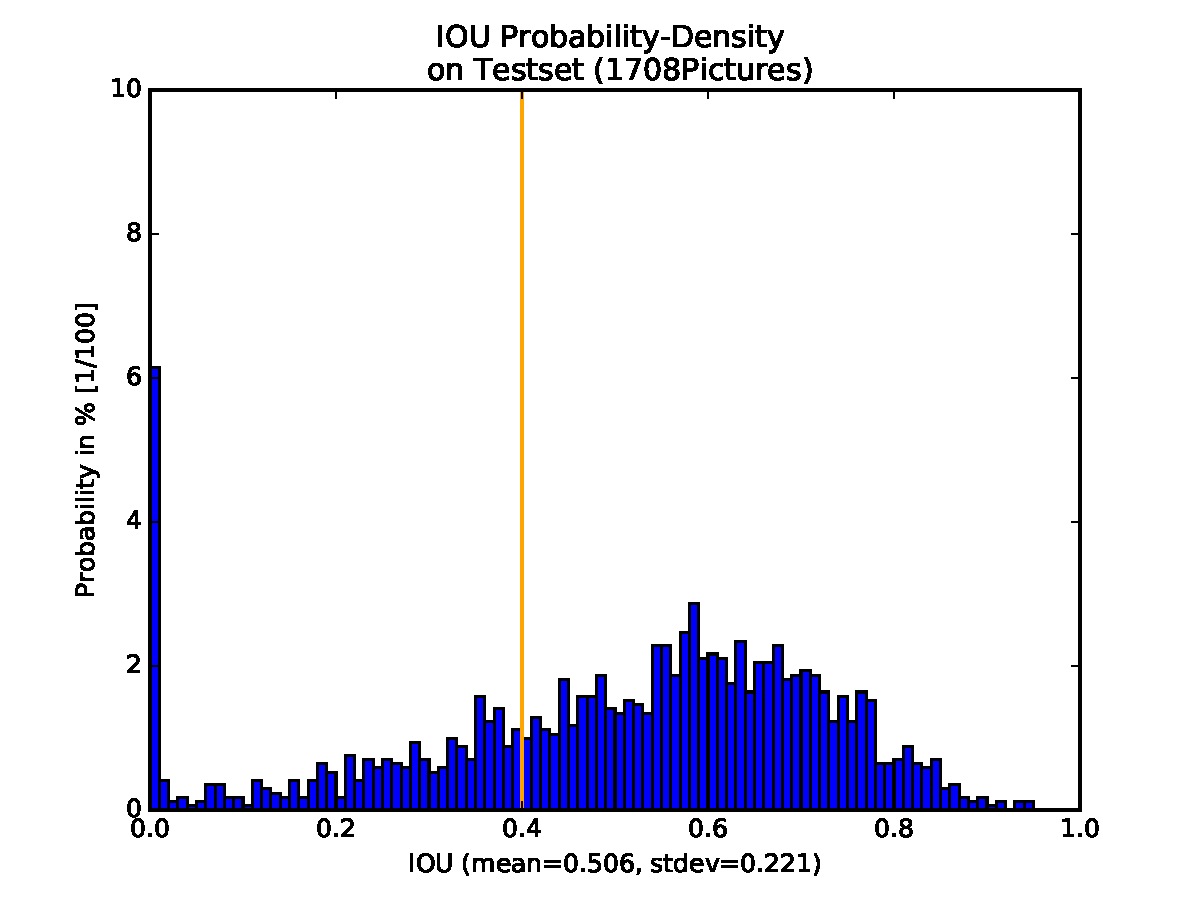
\includegraphics[width=.7\textwidth]{Kapitel/Resultate/Bilder/IOUprobDensity.pdf}
	\caption{Wahrscheinlichkeits-Dichte-Funktion der IOU (Grenze: IOU=0.4)}
	\label{img:iou_dichte}
\end{figure}


Die IOU beschreibt die Überlappung der vorhergesagten Boundingbox und der Boundingbox des Labels. 
Daher sagt die IOU einerseits etwas über die korrekte Grösse der Boundingbox, sowie deren korrekte Lage aus. 
Um wieder etwas über gut und schlecht aussagen zu können, wurde wieder ein Threshold definiert (0.4).
Da durch die IOU wie erwähnt mehrere Faktoren beschrieben werden, ist die Grenze verschwommener. 
So gibt es nach menschlicher Ansicht hervorragende Vorhersagen, welche eine IOU von 0.3 haben und wiederum mässige Vorhersagen mit einer IOU von nahezu 0.4.
Um ein Gefühl für diesen Threshold zu kriegen lohnt es sich die Abbildungen \ref{img:iou_knapp_gut} \& \ref{img:iou_knapp_schlecht} zu berücksichtigen.
So fiel die Entscheidung den Threshold konservativ zu wählen, sodass nur Werte als gut erachtet werden könne, welche auch gut sind. 

Auch für die IOU gibt es zur Übersicht eine Wahrscheinlichkeitsdichte die in Abbildung \ref{img:iou_dichte} betrachtet werden kann.
Aus dieser Grafik kann gelesen werden, dass rund 18\% der Vorhersagen klar falsch sind, weil die IOU nur null ist, wenn sich die beiden Boundingboxen nicht berühren. Entsprechend kann gesagt werden, dass rund 82\% der vorhersagen zumindest sehr grob richtig sind, weil sich bei diesen 82\% die Boundingboxen von Label und Prediction zumindest ein ganz kleines bisschen überlappen. 
